\documentclass[twoside]{book}

% Packages required by doxygen
\usepackage{fixltx2e}
\usepackage{calc}
\usepackage{doxygen}
\usepackage[export]{adjustbox} % also loads graphicx
\usepackage{graphicx}
\usepackage[utf8]{inputenc}
\usepackage{makeidx}
\usepackage{multicol}
\usepackage{multirow}
\PassOptionsToPackage{warn}{textcomp}
\usepackage{textcomp}
\usepackage[nointegrals]{wasysym}
\usepackage[table]{xcolor}

% NLS support packages
\usepackage{polski}
\usepackage[T1]{fontenc}

% Font selection
\usepackage[T1]{fontenc}
\usepackage[scaled=.90]{helvet}
\usepackage{courier}
\usepackage{amssymb}
\usepackage{sectsty}
\renewcommand{\familydefault}{\sfdefault}
\allsectionsfont{%
  \fontseries{bc}\selectfont%
  \color{darkgray}%
}
\renewcommand{\DoxyLabelFont}{%
  \fontseries{bc}\selectfont%
  \color{darkgray}%
}
\newcommand{\+}{\discretionary{\mbox{\scriptsize$\hookleftarrow$}}{}{}}

% Page & text layout
\usepackage{geometry}
\geometry{%
  a4paper,%
  top=2.5cm,%
  bottom=2.5cm,%
  left=2.5cm,%
  right=2.5cm%
}
\tolerance=750
\hfuzz=15pt
\hbadness=750
\setlength{\emergencystretch}{15pt}
\setlength{\parindent}{0cm}
\setlength{\parskip}{0.2cm}
\makeatletter
\renewcommand{\paragraph}{%
  \@startsection{paragraph}{4}{0ex}{-1.0ex}{1.0ex}{%
    \normalfont\normalsize\bfseries\SS@parafont%
  }%
}
\renewcommand{\subparagraph}{%
  \@startsection{subparagraph}{5}{0ex}{-1.0ex}{1.0ex}{%
    \normalfont\normalsize\bfseries\SS@subparafont%
  }%
}
\makeatother

% Headers & footers
\usepackage{fancyhdr}
\pagestyle{fancyplain}
\fancyhead[LE]{\fancyplain{}{\bfseries\thepage}}
\fancyhead[CE]{\fancyplain{}{}}
\fancyhead[RE]{\fancyplain{}{\bfseries\leftmark}}
\fancyhead[LO]{\fancyplain{}{\bfseries\rightmark}}
\fancyhead[CO]{\fancyplain{}{}}
\fancyhead[RO]{\fancyplain{}{\bfseries\thepage}}
\fancyfoot[LE]{\fancyplain{}{}}
\fancyfoot[CE]{\fancyplain{}{}}
\fancyfoot[RE]{\fancyplain{}{\bfseries\scriptsize Wygenerowano Pn, 4 kwi 2016 02\+:18\+:52 dla P\+A\+M\+S\+I 4 programem Doxygen }}
\fancyfoot[LO]{\fancyplain{}{\bfseries\scriptsize Wygenerowano Pn, 4 kwi 2016 02\+:18\+:52 dla P\+A\+M\+S\+I 4 programem Doxygen }}
\fancyfoot[CO]{\fancyplain{}{}}
\fancyfoot[RO]{\fancyplain{}{}}
\renewcommand{\footrulewidth}{0.4pt}
\renewcommand{\chaptermark}[1]{%
  \markboth{#1}{}%
}
\renewcommand{\sectionmark}[1]{%
  \markright{\thesection\ #1}%
}

% Indices & bibliography
\usepackage{natbib}
\usepackage[titles]{tocloft}
\setcounter{tocdepth}{3}
\setcounter{secnumdepth}{5}
\makeindex

% Custom commands
\newcommand{\clearemptydoublepage}{%
  \newpage{\pagestyle{empty}\cleardoublepage}%
}


%===== C O N T E N T S =====

\begin{document}

% Titlepage & ToC
\pagenumbering{roman}
\begin{titlepage}
\vspace*{7cm}
\begin{center}%
{\Large P\+A\+M\+S\+I 4 \\[1ex]\large 4 }\\
\vspace*{1cm}
{\large Wygenerowano przez Doxygen 1.8.9.1}\\
\vspace*{0.5cm}
{\small Pn, 4 kwi 2016 02:18:52}\\
\end{center}
\end{titlepage}
\clearemptydoublepage
\tableofcontents
\clearemptydoublepage
\pagenumbering{arabic}

%--- Begin generated contents ---
\chapter{Indeks hierarchiczny}
\section{Hierarchia klas}
Ta lista dziedziczenia posortowana jest z grubsza, choć nie całkowicie, alfabetycznie\+:\begin{DoxyCompactList}
\item \contentsline{section}{tablica\+:\+:bad\+\_\+index}{\pageref{classtablica_1_1bad__index}}{}
\item \contentsline{section}{tablica\+:\+:empty}{\pageref{classtablica_1_1empty}}{}
\item \contentsline{section}{in\+Kolejka}{\pageref{classin_kolejka}}{}
\begin{DoxyCompactList}
\item \contentsline{section}{kolejka}{\pageref{classkolejka}}{}
\end{DoxyCompactList}
\item \contentsline{section}{in\+Lista}{\pageref{classin_lista}}{}
\begin{DoxyCompactList}
\item \contentsline{section}{lista}{\pageref{classlista}}{}
\item \contentsline{section}{listatest}{\pageref{classlistatest}}{}
\end{DoxyCompactList}
\item \contentsline{section}{in\+Stos}{\pageref{classin_stos}}{}
\begin{DoxyCompactList}
\item \contentsline{section}{stos}{\pageref{classstos}}{}
\end{DoxyCompactList}
\item \contentsline{section}{in\+Tablica}{\pageref{classin_tablica}}{}
\begin{DoxyCompactList}
\item \contentsline{section}{tablica}{\pageref{classtablica}}{}
\begin{DoxyCompactList}
\item \contentsline{section}{kolejka}{\pageref{classkolejka}}{}
\item \contentsline{section}{lista}{\pageref{classlista}}{}
\item \contentsline{section}{stos}{\pageref{classstos}}{}
\end{DoxyCompactList}
\item \contentsline{section}{tablica}{\pageref{classtablica}}{}
\end{DoxyCompactList}
\item \contentsline{section}{i\+Runnable}{\pageref{classi_runnable}}{}
\begin{DoxyCompactList}
\item \contentsline{section}{tablica}{\pageref{classtablica}}{}
\end{DoxyCompactList}
\item \contentsline{section}{stoper}{\pageref{classstoper}}{}
\item tablicatest\begin{DoxyCompactList}
\item \contentsline{section}{listatest}{\pageref{classlistatest}}{}
\end{DoxyCompactList}
\end{DoxyCompactList}

\chapter{Indeks klas}
\section{Lista klas}
Tutaj znajdują się klasy, struktury, unie i interfejsy wraz z ich krótkimi opisami\+:\begin{DoxyCompactList}
\item\contentsline{section}{{\bf tablica\+::bad\+\_\+index} \\*Obiekt zwracany podczas wystapienia wyjatku wystepujacego gdy nastapi proba odzialywania na dane ktorych kontener nie posiada }{\pageref{classtablica_1_1bad__index}}{}
\item\contentsline{section}{{\bf tablica\+::empty} \\*Metoda sprawdza czy kontener jest pusty }{\pageref{classtablica_1_1empty}}{}
\item\contentsline{section}{{\bf in\+Kolejka} }{\pageref{classin_kolejka}}{}
\item\contentsline{section}{{\bf in\+Lista} }{\pageref{classin_lista}}{}
\item\contentsline{section}{{\bf in\+Stos} }{\pageref{classin_stos}}{}
\item\contentsline{section}{{\bf in\+Tablica} }{\pageref{classin_tablica}}{}
\item\contentsline{section}{{\bf i\+Runnable} }{\pageref{classi_runnable}}{}
\item\contentsline{section}{{\bf kolejka} }{\pageref{classkolejka}}{}
\item\contentsline{section}{{\bf lista} }{\pageref{classlista}}{}
\item\contentsline{section}{{\bf listatest} }{\pageref{classlistatest}}{}
\item\contentsline{section}{{\bf stoper} }{\pageref{classstoper}}{}
\item\contentsline{section}{{\bf stos} }{\pageref{classstos}}{}
\item\contentsline{section}{{\bf tablica} }{\pageref{classtablica}}{}
\end{DoxyCompactList}

\chapter{Indeks plików}
\section{Lista plików}
Tutaj znajduje się lista wszystkich plików z ich krótkimi opisami\+:\begin{DoxyCompactList}
\item\contentsline{section}{\hyperlink{atp_8hh}{atp.\+hh} }{\pageref{atp_8hh}}{}
\item\contentsline{section}{\hyperlink{atp2_8hh}{atp2.\+hh} \\*Plik zawiera definicje klasy wirtualnej \hyperlink{classatp2}{atp2} z ktorej skladaja sie zaimplementowane abstrakcyjne typy danych }{\pageref{atp2_8hh}}{}
\item\contentsline{section}{\hyperlink{irunnable_8hh}{irunnable.\+hh} }{\pageref{irunnable_8hh}}{}
\item\contentsline{section}{\hyperlink{kolejka_8cpp}{kolejka.\+cpp} }{\pageref{kolejka_8cpp}}{}
\item\contentsline{section}{\hyperlink{kolejka_8hh}{kolejka.\+hh} \\*Plik zawiera definicje klasy kolejka }{\pageref{kolejka_8hh}}{}
\item\contentsline{section}{\hyperlink{lista_8cpp}{lista.\+cpp} }{\pageref{lista_8cpp}}{}
\item\contentsline{section}{\hyperlink{lista_8hh}{lista.\+hh} \\*Plik zawiera klase lista }{\pageref{lista_8hh}}{}
\item\contentsline{section}{\hyperlink{main_8cpp}{main.\+cpp} }{\pageref{main_8cpp}}{}
\item\contentsline{section}{\hyperlink{stoper_8cpp}{stoper.\+cpp} }{\pageref{stoper_8cpp}}{}
\item\contentsline{section}{\hyperlink{stoper_8hh}{stoper.\+hh} }{\pageref{stoper_8hh}}{}
\item\contentsline{section}{\hyperlink{stos_8cpp}{stos.\+cpp} }{\pageref{stos_8cpp}}{}
\item\contentsline{section}{\hyperlink{stos_8hh}{stos.\+hh} \\*Plik zawiera definicje klasy stos }{\pageref{stos_8hh}}{}
\item\contentsline{section}{\hyperlink{tablica_8cpp}{tablica.\+cpp} }{\pageref{tablica_8cpp}}{}
\item\contentsline{section}{\hyperlink{tablica_8hh}{tablica.\+hh} \\*Plik zawiera klase tablica }{\pageref{tablica_8hh}}{}
\end{DoxyCompactList}

\chapter{Dokumentacja klas}
\section{Dokumentacja klasy tablica\+:\+:bad\+\_\+index}
\label{classtablica_1_1bad__index}\index{tablica\+::bad\+\_\+index@{tablica\+::bad\+\_\+index}}


obiekt zwracany podczas wystapienia wyjatku wystepujacego gdy nastapi proba odzialywania na dane ktorych kontener nie posiada  




{\ttfamily \#include $<$tablica.\+hh$>$}



\subsection{Opis szczegółowy}
obiekt zwracany podczas wystapienia wyjatku wystepujacego gdy nastapi proba odzialywania na dane ktorych kontener nie posiada 

Dokumentacja dla tej klasy została wygenerowana z pliku\+:\begin{DoxyCompactItemize}
\item 
inc/{\bf tablica.\+hh}\end{DoxyCompactItemize}

\section{Dokumentacja klasy tablica\+:\+:empty}
\label{classtablica_1_1empty}\index{tablica\+::empty@{tablica\+::empty}}


metoda sprawdza czy kontener jest pusty  




{\ttfamily \#include $<$tablica.\+hh$>$}



\subsection{Opis szczegółowy}
metoda sprawdza czy kontener jest pusty 

Dokumentacja dla tej klasy została wygenerowana z pliku\+:\begin{DoxyCompactItemize}
\item 
inc/{\bf tablica.\+hh}\end{DoxyCompactItemize}

\section{Dokumentacja klasy in\+Kolejka}
\label{classin_kolejka}\index{in\+Kolejka@{in\+Kolejka}}


Diagram dziedziczenia dla in\+Kolejka
\nopagebreak
\begin{figure}[H]
\begin{center}
\leavevmode
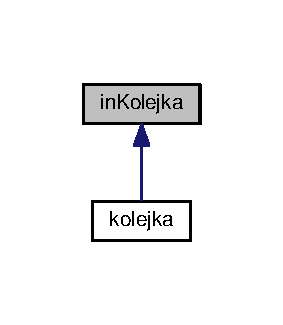
\includegraphics[width=136pt]{classin_kolejka__inherit__graph}
\end{center}
\end{figure}
\subsection*{Metody publiczne}
\begin{DoxyCompactItemize}
\item 
virtual void {\bfseries remove} ()=0\label{classin_kolejka_ac5cab7b3ed5f6d2ecdd0b56b49052c3d}

\item 
virtual void {\bfseries add} (int)=0\label{classin_kolejka_a44867628b735e9896251879866424132}

\item 
virtual int {\bfseries last} ()=0\label{classin_kolejka_a378039173f692c438912890d247036ee}

\item 
virtual int {\bfseries first} ()=0\label{classin_kolejka_aee5f6ffb249dc8284fb659d73f5f2ed6}

\end{DoxyCompactItemize}


Dokumentacja dla tej klasy została wygenerowana z pliku\+:\begin{DoxyCompactItemize}
\item 
inc/inkolejka.\+hh\end{DoxyCompactItemize}

\section{Dokumentacja klasy in\+Lista}
\label{classin_lista}\index{in\+Lista@{in\+Lista}}


Diagram dziedziczenia dla in\+Lista
\nopagebreak
\begin{figure}[H]
\begin{center}
\leavevmode
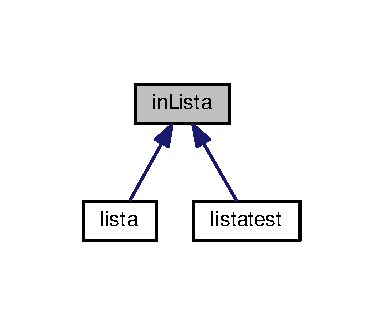
\includegraphics[width=184pt]{classin_lista__inherit__graph}
\end{center}
\end{figure}
\subsection*{Metody publiczne}
\begin{DoxyCompactItemize}
\item 
virtual void {\bfseries remove} (int)=0\label{classin_lista_abfa8aec6ac57b58ab0d890038d722e2e}

\item 
virtual void {\bfseries remove} ()=0\label{classin_lista_a6c153759e6ddb28590bdd13aa3e6e995}

\item 
virtual void {\bfseries add} (int, int)=0\label{classin_lista_a5086e60e89b9eb884219190c38daa9bd}

\item 
virtual void {\bfseries add} (int)=0\label{classin_lista_a6308248620986ae04e828f8a1ecde258}

\item 
virtual int {\bfseries get} (int)=0\label{classin_lista_a55ba3ad03b786ee930ba83c9b1c89fa4}

\end{DoxyCompactItemize}


Dokumentacja dla tej klasy została wygenerowana z pliku\+:\begin{DoxyCompactItemize}
\item 
inc/inlista.\+hh\end{DoxyCompactItemize}

\section{Dokumentacja klasy in\+Stos}
\label{classin_stos}\index{in\+Stos@{in\+Stos}}


Diagram dziedziczenia dla in\+Stos
\nopagebreak
\begin{figure}[H]
\begin{center}
\leavevmode
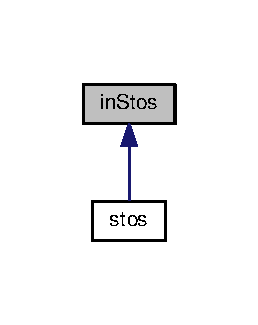
\includegraphics[width=124pt]{classin_stos__inherit__graph}
\end{center}
\end{figure}
\subsection*{Metody publiczne}
\begin{DoxyCompactItemize}
\item 
virtual void {\bfseries remove} ()=0\label{classin_stos_a8cbd9941b251f12f8dbead239f5117e8}

\item 
virtual void {\bfseries add} (int)=0\label{classin_stos_a4eec0b97e9e0e7043decb1b39cd9da4b}

\item 
virtual int {\bfseries get} ()=0\label{classin_stos_a7caf60f2603a69cdee579ababf61e021}

\end{DoxyCompactItemize}


Dokumentacja dla tej klasy została wygenerowana z pliku\+:\begin{DoxyCompactItemize}
\item 
inc/instos.\+hh\end{DoxyCompactItemize}

\section{Dokumentacja klasy in\+Tablica}
\label{classin_tablica}\index{in\+Tablica@{in\+Tablica}}


Diagram dziedziczenia dla in\+Tablica
\nopagebreak
\begin{figure}[H]
\begin{center}
\leavevmode
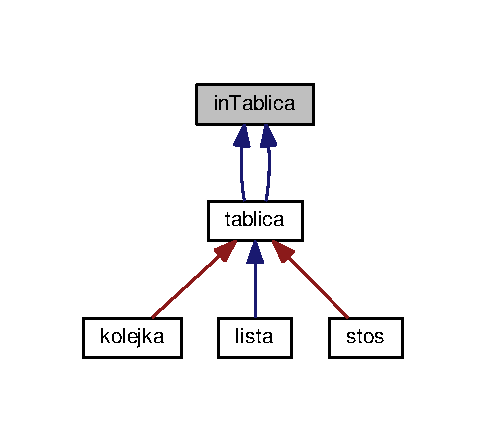
\includegraphics[width=233pt]{classin_tablica__inherit__graph}
\end{center}
\end{figure}
\subsection*{Metody publiczne}
\begin{DoxyCompactItemize}
\item 
virtual void {\bfseries push} (int)=0\label{classin_tablica_a9ba9ffcda633d7788acbbc877b402d2e}

\item 
virtual void {\bfseries przypisz} (int, int)=0\label{classin_tablica_a0261e4203277dc7bb509a6e16ea11fee}

\item 
virtual void {\bfseries zdejmij} (int)=0\label{classin_tablica_a1e01ff840ff32352abac3c2b4b8de684}

\item 
virtual int {\bfseries size} ()=0\label{classin_tablica_a039fb28e7e83fb730a45050a8b43847f}

\item 
virtual int {\bfseries ind} ()=0\label{classin_tablica_a58a123a9dfc74fcfe7ce824a228c2153}

\item 
virtual bool {\bfseries is\+Empty} ()=0\label{classin_tablica_a29cd0f3dffa632a9a54a64079eae9019}

\end{DoxyCompactItemize}


Dokumentacja dla tej klasy została wygenerowana z pliku\+:\begin{DoxyCompactItemize}
\item 
inc/intablica.\+hh\end{DoxyCompactItemize}

\hypertarget{classi_runnable}{}\section{Dokumentacja klasy i\+Runnable}
\label{classi_runnable}\index{i\+Runnable@{i\+Runnable}}


{\ttfamily \#include $<$irunnable.\+hh$>$}

\subsection*{Metody publiczne}
\begin{DoxyCompactItemize}
\item 
bool \hyperlink{classi_runnable_a552d10b91924fefc6ef0bfc7cb1ff66a}{run} ()
\item 
bool \hyperlink{classi_runnable_adaa50510fc6965174a7b871f87feb1e5}{prepare} ()
\end{DoxyCompactItemize}


\subsection{Opis szczegółowy}


Definicja w linii 3 pliku irunnable.\+hh.



\subsection{Dokumentacja funkcji składowych}
\hypertarget{classi_runnable_adaa50510fc6965174a7b871f87feb1e5}{}\index{i\+Runnable@{i\+Runnable}!prepare@{prepare}}
\index{prepare@{prepare}!i\+Runnable@{i\+Runnable}}
\subsubsection[{prepare}]{\setlength{\rightskip}{0pt plus 5cm}bool i\+Runnable\+::prepare (
\begin{DoxyParamCaption}
{}
\end{DoxyParamCaption}
)}\label{classi_runnable_adaa50510fc6965174a7b871f87feb1e5}
\hypertarget{classi_runnable_a552d10b91924fefc6ef0bfc7cb1ff66a}{}\index{i\+Runnable@{i\+Runnable}!run@{run}}
\index{run@{run}!i\+Runnable@{i\+Runnable}}
\subsubsection[{run}]{\setlength{\rightskip}{0pt plus 5cm}bool i\+Runnable\+::run (
\begin{DoxyParamCaption}
{}
\end{DoxyParamCaption}
)}\label{classi_runnable_a552d10b91924fefc6ef0bfc7cb1ff66a}


Dokumentacja dla tej klasy została wygenerowana z pliku\+:\begin{DoxyCompactItemize}
\item 
\hyperlink{irunnable_8hh}{irunnable.\+hh}\end{DoxyCompactItemize}

\section{Dokumentacja klasy kolejka}
\label{classkolejka}\index{kolejka@{kolejka}}


Diagram dziedziczenia dla kolejka
\nopagebreak
\begin{figure}[H]
\begin{center}
\leavevmode
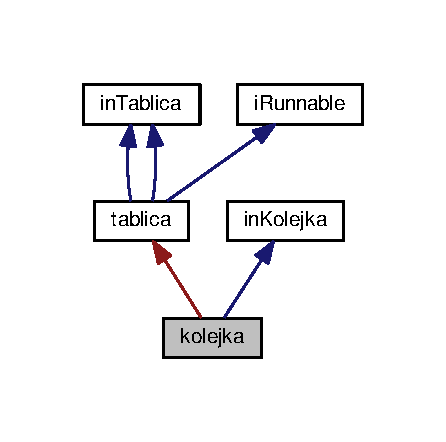
\includegraphics[width=214pt]{classkolejka__inherit__graph}
\end{center}
\end{figure}


Diagram współpracy dla kolejka\+:
\nopagebreak
\begin{figure}[H]
\begin{center}
\leavevmode
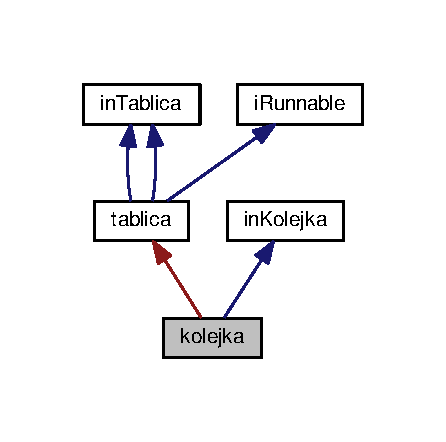
\includegraphics[width=214pt]{classkolejka__coll__graph}
\end{center}
\end{figure}
\subsection*{Metody publiczne}
\begin{DoxyCompactItemize}
\item 
{\bf kolejka} ()
\begin{DoxyCompactList}\small\item\em Klasa kolejka -\/ jeden z abstrakcyjnych typow danych. \end{DoxyCompactList}\item 
void {\bfseries remove} ()\label{classkolejka_a38392eb78d5c659ed90aff8a8d8b078d}

\item 
void {\bf add} (int)\label{classkolejka_a2b9a60c6e42764a419e6e7347c2f4227}

\begin{DoxyCompactList}\small\item\em usuwa pierwsza dana w kolejce \end{DoxyCompactList}\item 
int {\bf first} ()\label{classkolejka_a0c4bda6901284547852147a9a4f2d2f5}

\begin{DoxyCompactList}\small\item\em dodaje dana na koniec kolejki \end{DoxyCompactList}\item 
int {\bf last} ()\label{classkolejka_ac901b09064b29221205d37bb5d822c93}

\begin{DoxyCompactList}\small\item\em zwraca wartosc pierwszej danej \end{DoxyCompactList}\end{DoxyCompactItemize}


\subsection{Dokumentacja konstruktora i destruktora}
\index{kolejka@{kolejka}!kolejka@{kolejka}}
\index{kolejka@{kolejka}!kolejka@{kolejka}}
\subsubsection[{kolejka}]{\setlength{\rightskip}{0pt plus 5cm}kolejka\+::kolejka (
\begin{DoxyParamCaption}
{}
\end{DoxyParamCaption}
)}\label{classkolejka_ae9205d86a1f136649fac28615878729c}


Klasa kolejka -\/ jeden z abstrakcyjnych typow danych. 

Klasa ma w swoim skladzie metody sluzace do zarzadzania kolejka, wszytskie operacje poza dodaniem nowej danej do pustej kolejki zglaszaja wyjatek 

Dokumentacja dla tej klasy została wygenerowana z plików\+:\begin{DoxyCompactItemize}
\item 
inc/{\bf kolejka.\+hh}\item 
src/kolejka.\+cpp\end{DoxyCompactItemize}

\hypertarget{classlista}{}\section{Dokumentacja klasy lista}
\label{classlista}\index{lista@{lista}}


{\ttfamily \#include $<$lista.\+hh$>$}



Diagram dziedziczenia dla lista\nopagebreak
\begin{figure}[H]
\begin{center}
\leavevmode
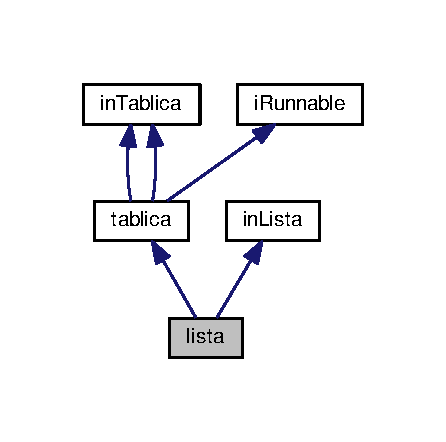
\includegraphics[width=125pt]{classlista__inherit__graph}
\end{center}
\end{figure}


Diagram współpracy dla lista\+:\nopagebreak
\begin{figure}[H]
\begin{center}
\leavevmode
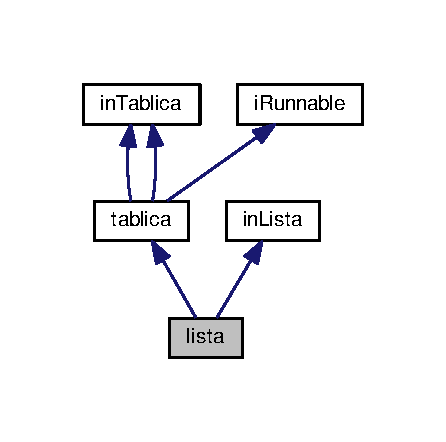
\includegraphics[width=125pt]{classlista__coll__graph}
\end{center}
\end{figure}
\subsection*{Metody publiczne}
\begin{DoxyCompactItemize}
\item 
\hyperlink{classlista_a7ae1e1582d5b90e6bc26b8ecd2894072}{lista} ()
\item 
void \hyperlink{classlista_a567ac3ce85a3a7d7b10a3b0aafed56dd}{remove} (int)
\item 
void \hyperlink{classlista_af1900e0adeee6f2bf55c3b01c94b5e42}{remove} ()
\begin{DoxyCompactList}\small\item\em usuwa dana o podanym indeksie, a nastepnie przestawia zmienne \end{DoxyCompactList}\item 
void \hyperlink{classlista_abbc313e4d15605053e317b28246146bf}{add} (int, int)
\begin{DoxyCompactList}\small\item\em usuwa ostatnia dana w kolejce \end{DoxyCompactList}\item 
void \hyperlink{classlista_aa3b586da2830b20ca5818509a34ed6a6}{add} (int)
\begin{DoxyCompactList}\small\item\em dodaje dana na miejscu o podanym indeksie, jezeli nie moze byc tam wstawiona zglosi wyjatek, gdy miejsce jest zajete przestawia dane \end{DoxyCompactList}\item 
int \hyperlink{classlista_aca7a3313138e7033678c32b625fd5473}{get} (int)
\begin{DoxyCompactList}\small\item\em dodaje dana na koniec listy \end{DoxyCompactList}\end{DoxyCompactItemize}
\subsection*{Dodatkowe Dziedziczone Składowe}


\subsection{Opis szczegółowy}


Definicja w linii 8 pliku lista.\+hh.



\subsection{Dokumentacja konstruktora i destruktora}
\hypertarget{classlista_a7ae1e1582d5b90e6bc26b8ecd2894072}{}\index{lista@{lista}!lista@{lista}}
\index{lista@{lista}!lista@{lista}}
\subsubsection[{lista}]{\setlength{\rightskip}{0pt plus 5cm}lista\+::lista (
\begin{DoxyParamCaption}
{}
\end{DoxyParamCaption}
)}\label{classlista_a7ae1e1582d5b90e6bc26b8ecd2894072}


Definicja w linii 3 pliku lista.\+cpp.



\subsection{Dokumentacja funkcji składowych}
\hypertarget{classlista_abbc313e4d15605053e317b28246146bf}{}\index{lista@{lista}!add@{add}}
\index{add@{add}!lista@{lista}}
\subsubsection[{add}]{\setlength{\rightskip}{0pt plus 5cm}void lista\+::add (
\begin{DoxyParamCaption}
\item[{int}]{x, }
\item[{int}]{index}
\end{DoxyParamCaption}
)}\label{classlista_abbc313e4d15605053e317b28246146bf}


usuwa ostatnia dana w kolejce 



Definicja w linii 10 pliku lista.\+cpp.



Oto graf wywołań dla tej funkcji\+:\nopagebreak
\begin{figure}[H]
\begin{center}
\leavevmode
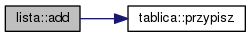
\includegraphics[width=260pt]{classlista_abbc313e4d15605053e317b28246146bf_cgraph}
\end{center}
\end{figure}




Oto graf wywoływań tej funkcji\+:\nopagebreak
\begin{figure}[H]
\begin{center}
\leavevmode
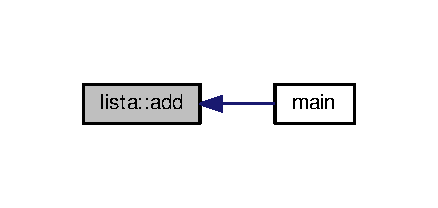
\includegraphics[width=210pt]{classlista_abbc313e4d15605053e317b28246146bf_icgraph}
\end{center}
\end{figure}


\hypertarget{classlista_aa3b586da2830b20ca5818509a34ed6a6}{}\index{lista@{lista}!add@{add}}
\index{add@{add}!lista@{lista}}
\subsubsection[{add}]{\setlength{\rightskip}{0pt plus 5cm}void lista\+::add (
\begin{DoxyParamCaption}
\item[{int}]{x}
\end{DoxyParamCaption}
)\hspace{0.3cm}{\ttfamily [virtual]}}\label{classlista_aa3b586da2830b20ca5818509a34ed6a6}


dodaje dana na miejscu o podanym indeksie, jezeli nie moze byc tam wstawiona zglosi wyjatek, gdy miejsce jest zajete przestawia dane 



Implementuje \hyperlink{classatp_a1952565164abe3c3ddd8ab78a152ff0a}{atp}.



Definicja w linii 6 pliku lista.\+cpp.



Oto graf wywołań dla tej funkcji\+:\nopagebreak
\begin{figure}[H]
\begin{center}
\leavevmode
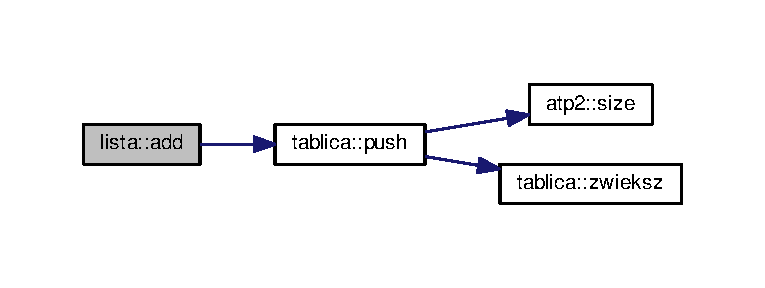
\includegraphics[width=350pt]{classlista_aa3b586da2830b20ca5818509a34ed6a6_cgraph}
\end{center}
\end{figure}


\hypertarget{classlista_aca7a3313138e7033678c32b625fd5473}{}\index{lista@{lista}!get@{get}}
\index{get@{get}!lista@{lista}}
\subsubsection[{get}]{\setlength{\rightskip}{0pt plus 5cm}int lista\+::get (
\begin{DoxyParamCaption}
\item[{int}]{i}
\end{DoxyParamCaption}
)\hspace{0.3cm}{\ttfamily [virtual]}}\label{classlista_aca7a3313138e7033678c32b625fd5473}


dodaje dana na koniec listy 



Implementuje \hyperlink{classatp_a983ada7a72bc51ef2097a74022c8985c}{atp}.



Definicja w linii 33 pliku lista.\+cpp.



Oto graf wywołań dla tej funkcji\+:\nopagebreak
\begin{figure}[H]
\begin{center}
\leavevmode
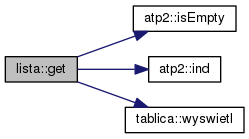
\includegraphics[width=259pt]{classlista_aca7a3313138e7033678c32b625fd5473_cgraph}
\end{center}
\end{figure}




Oto graf wywoływań tej funkcji\+:\nopagebreak
\begin{figure}[H]
\begin{center}
\leavevmode
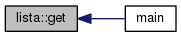
\includegraphics[width=208pt]{classlista_aca7a3313138e7033678c32b625fd5473_icgraph}
\end{center}
\end{figure}


\hypertarget{classlista_a567ac3ce85a3a7d7b10a3b0aafed56dd}{}\index{lista@{lista}!remove@{remove}}
\index{remove@{remove}!lista@{lista}}
\subsubsection[{remove}]{\setlength{\rightskip}{0pt plus 5cm}void lista\+::remove (
\begin{DoxyParamCaption}
\item[{int}]{i}
\end{DoxyParamCaption}
)}\label{classlista_a567ac3ce85a3a7d7b10a3b0aafed56dd}


Definicja w linii 17 pliku lista.\+cpp.



Oto graf wywołań dla tej funkcji\+:\nopagebreak
\begin{figure}[H]
\begin{center}
\leavevmode
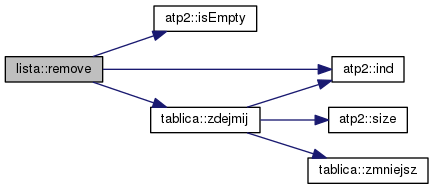
\includegraphics[width=350pt]{classlista_a567ac3ce85a3a7d7b10a3b0aafed56dd_cgraph}
\end{center}
\end{figure}


\hypertarget{classlista_af1900e0adeee6f2bf55c3b01c94b5e42}{}\index{lista@{lista}!remove@{remove}}
\index{remove@{remove}!lista@{lista}}
\subsubsection[{remove}]{\setlength{\rightskip}{0pt plus 5cm}void lista\+::remove (
\begin{DoxyParamCaption}
{}
\end{DoxyParamCaption}
)\hspace{0.3cm}{\ttfamily [virtual]}}\label{classlista_af1900e0adeee6f2bf55c3b01c94b5e42}


usuwa dana o podanym indeksie, a nastepnie przestawia zmienne 



Implementuje \hyperlink{classatp_a8294b0364a83890f88ef798b11473f7e}{atp}.



Definicja w linii 26 pliku lista.\+cpp.



Oto graf wywołań dla tej funkcji\+:\nopagebreak
\begin{figure}[H]
\begin{center}
\leavevmode
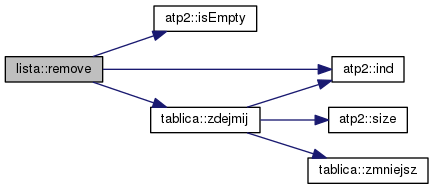
\includegraphics[width=350pt]{classlista_af1900e0adeee6f2bf55c3b01c94b5e42_cgraph}
\end{center}
\end{figure}




Dokumentacja dla tej klasy została wygenerowana z plików\+:\begin{DoxyCompactItemize}
\item 
\hyperlink{lista_8hh}{lista.\+hh}\item 
\hyperlink{lista_8cpp}{lista.\+cpp}\end{DoxyCompactItemize}

\section{Dokumentacja klasy listatest}
\label{classlistatest}\index{listatest@{listatest}}


Diagram dziedziczenia dla listatest
\nopagebreak
\begin{figure}[H]
\begin{center}
\leavevmode
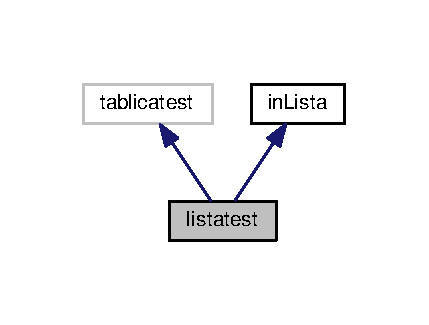
\includegraphics[width=206pt]{classlistatest__inherit__graph}
\end{center}
\end{figure}


Diagram współpracy dla listatest\+:
\nopagebreak
\begin{figure}[H]
\begin{center}
\leavevmode
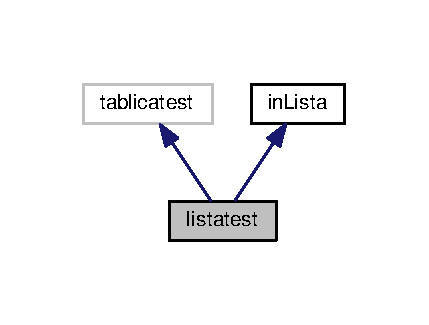
\includegraphics[width=206pt]{classlistatest__coll__graph}
\end{center}
\end{figure}
\subsection*{Metody publiczne}
\begin{DoxyCompactItemize}
\item 
{\bfseries lista} ()\label{classlistatest_ab68d3f591f7919c48ff11ecc954e5bfc}

\item 
void {\bfseries remove} (int)\label{classlistatest_a72670c086c60d2f5eb907021b08f6832}

\item 
void {\bf remove} ()\label{classlistatest_a68f3e4576befef3f0c87d0d267b62607}

\begin{DoxyCompactList}\small\item\em usuwa dana o podanym indeksie, a nastepnie przestawia zmienne \end{DoxyCompactList}\item 
void {\bf add} (int, int)\label{classlistatest_a5f0649c070d004ba76f9107228e610fb}

\begin{DoxyCompactList}\small\item\em usuwa ostatnia dana w kolejce \end{DoxyCompactList}\item 
void {\bf add} (int)\label{classlistatest_af7049706d52168c353a6cdf7f5df23b7}

\begin{DoxyCompactList}\small\item\em dodaje dana na miejscu o podanym indeksie, jezeli nie moze byc tam wstawiona zglosi wyjatek, gdy miejsce jest zajete przestawia dane \end{DoxyCompactList}\item 
int {\bf get} (int)\label{classlistatest_ac6e515602f13c5a8823e45eeef948f01}

\begin{DoxyCompactList}\small\item\em dodaje dana na koniec listy \end{DoxyCompactList}\item 
void {\bf run} ()\label{classlistatest_a60205347050d77d5a1f224b3543395b7}

\begin{DoxyCompactList}\small\item\em zwraca wartosc na podanym indeksie, jezeli nie moze tego zrobic, zwroci wyjatek \end{DoxyCompactList}\end{DoxyCompactItemize}


Dokumentacja dla tej klasy została wygenerowana z plików\+:\begin{DoxyCompactItemize}
\item 
inc/{\bf listatest.\+hh}\item 
src/listatest.\+cpp\end{DoxyCompactItemize}

\section{Dokumentacja klasy stoper}
\label{classstoper}\index{stoper@{stoper}}
\subsection*{Metody publiczne}
\begin{DoxyCompactItemize}
\item 
void {\bfseries start} ()\label{classstoper_a8f639c24ef48d1d7a95fae60239838e6}

\item 
void {\bfseries stop} ()\label{classstoper_a6c35c886ee95dffbf254a917b50f08fa}

\item 
std\+::chrono\+::duration$<$ double $>$ {\bfseries get\+Elapsed\+Time} ()\label{classstoper_ac5f064a27dcf65edd9acc810e77f756a}

\item 
std\+::chrono\+::duration$<$ double $>$ {\bfseries get\+Time} ()\label{classstoper_a51914c2059ccd64fc169db0be354c404}

\item 
bool {\bfseries dump\+To\+File} (std\+::string)\label{classstoper_a9092eba4af7172dd26c3046dbff408f9}

\end{DoxyCompactItemize}


Dokumentacja dla tej klasy została wygenerowana z plików\+:\begin{DoxyCompactItemize}
\item 
inc/stoper.\+hh\item 
src/stoper.\+cpp\end{DoxyCompactItemize}

\hypertarget{classstos}{}\section{Dokumentacja klasy stos}
\label{classstos}\index{stos@{stos}}


{\ttfamily \#include $<$stos.\+hh$>$}



Diagram dziedziczenia dla stos\nopagebreak
\begin{figure}[H]
\begin{center}
\leavevmode
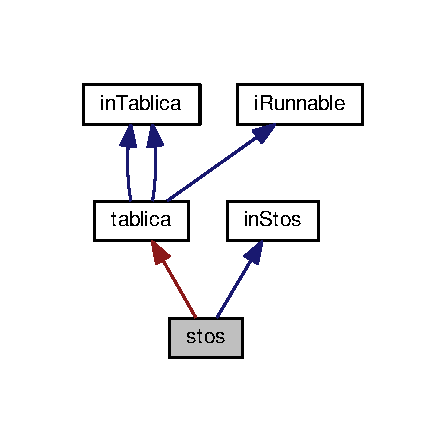
\includegraphics[width=125pt]{classstos__inherit__graph}
\end{center}
\end{figure}


Diagram współpracy dla stos\+:\nopagebreak
\begin{figure}[H]
\begin{center}
\leavevmode
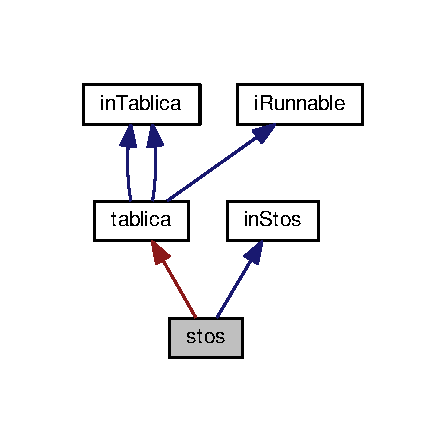
\includegraphics[width=125pt]{classstos__coll__graph}
\end{center}
\end{figure}
\subsection*{Metody publiczne}
\begin{DoxyCompactItemize}
\item 
\hyperlink{classstos_afb387ac69250038334f6d8099b6a2421}{stos} ()
\begin{DoxyCompactList}\small\item\em Klasa stos -\/ jeden z abstrakcyjnych typow danych. \end{DoxyCompactList}\item 
void \hyperlink{classstos_a8af2cbfa1b680a7f045d3390a46a1748}{remove} ()
\begin{DoxyCompactList}\small\item\em konstruktor bezparametryczny \end{DoxyCompactList}\item 
void \hyperlink{classstos_add60398fb259ecc3f64cd43c9c74422f}{add} (int)
\begin{DoxyCompactList}\small\item\em metoda \hyperlink{classstos_a8af2cbfa1b680a7f045d3390a46a1748}{remove()}-\/ nie przyjmuje wartosci, usuwa najwyzej polozona na stosie dana \end{DoxyCompactList}\item 
int \hyperlink{classstos_a5d1b9f3ae3c00298385b555113a7467a}{get} (int=0)
\begin{DoxyCompactList}\small\item\em metoda \hyperlink{classstos_add60398fb259ecc3f64cd43c9c74422f}{add(int)}-\/ przyjmuje wartosc int, bedaca nowa liczba do dodania na szczyt stosu \end{DoxyCompactList}\item 
int \hyperlink{classstos_a84a6713aeafdd62ef6fe51fa11b7b6fa}{get} ()
\begin{DoxyCompactList}\small\item\em metoda get z parametrem int nie powinna byc uzywana, mozliwe jest uzycie jedynie zerowego indeklu, wszystkie inne zwracaja wyjatek,bezpieczniej jest uzywac \hyperlink{classstos_a84a6713aeafdd62ef6fe51fa11b7b6fa}{get()} \end{DoxyCompactList}\end{DoxyCompactItemize}
\subsection*{Dodatkowe Dziedziczone Składowe}


\subsection{Opis szczegółowy}


Definicja w linii 8 pliku stos.\+hh.



\subsection{Dokumentacja konstruktora i destruktora}
\hypertarget{classstos_afb387ac69250038334f6d8099b6a2421}{}\index{stos@{stos}!stos@{stos}}
\index{stos@{stos}!stos@{stos}}
\subsubsection[{stos}]{\setlength{\rightskip}{0pt plus 5cm}stos\+::stos (
\begin{DoxyParamCaption}
{}
\end{DoxyParamCaption}
)}\label{classstos_afb387ac69250038334f6d8099b6a2421}


Klasa stos -\/ jeden z abstrakcyjnych typow danych. 

Klasa ma w swoim skladzie metody sluzace do zarzadzania stosem, mozliwe jest jedynie manipulowanie najwyzej polozonym elementem na stosie, inne operacje poza dodaniem nowej danej do niego na pustym stosie zglaszaja wyjatek 

Definicja w linii 3 pliku stos.\+cpp.



\subsection{Dokumentacja funkcji składowych}
\hypertarget{classstos_add60398fb259ecc3f64cd43c9c74422f}{}\index{stos@{stos}!add@{add}}
\index{add@{add}!stos@{stos}}
\subsubsection[{add}]{\setlength{\rightskip}{0pt plus 5cm}void stos\+::add (
\begin{DoxyParamCaption}
\item[{int}]{x}
\end{DoxyParamCaption}
)\hspace{0.3cm}{\ttfamily [virtual]}}\label{classstos_add60398fb259ecc3f64cd43c9c74422f}


metoda \hyperlink{classstos_a8af2cbfa1b680a7f045d3390a46a1748}{remove()}-\/ nie przyjmuje wartosci, usuwa najwyzej polozona na stosie dana 



Implementuje \hyperlink{classatp_a1952565164abe3c3ddd8ab78a152ff0a}{atp}.



Definicja w linii 5 pliku stos.\+cpp.



Oto graf wywołań dla tej funkcji\+:\nopagebreak
\begin{figure}[H]
\begin{center}
\leavevmode
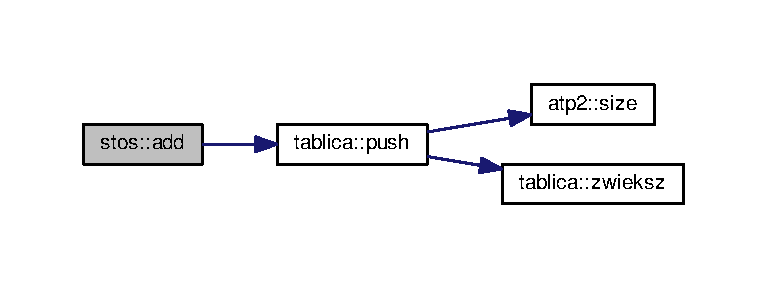
\includegraphics[width=350pt]{classstos_add60398fb259ecc3f64cd43c9c74422f_cgraph}
\end{center}
\end{figure}


\hypertarget{classstos_a5d1b9f3ae3c00298385b555113a7467a}{}\index{stos@{stos}!get@{get}}
\index{get@{get}!stos@{stos}}
\subsubsection[{get}]{\setlength{\rightskip}{0pt plus 5cm}int stos\+::get (
\begin{DoxyParamCaption}
\item[{int}]{i = {\ttfamily 0}}
\end{DoxyParamCaption}
)\hspace{0.3cm}{\ttfamily [virtual]}}\label{classstos_a5d1b9f3ae3c00298385b555113a7467a}


metoda \hyperlink{classstos_add60398fb259ecc3f64cd43c9c74422f}{add(int)}-\/ przyjmuje wartosc int, bedaca nowa liczba do dodania na szczyt stosu 



Implementuje \hyperlink{classatp_a983ada7a72bc51ef2097a74022c8985c}{atp}.



Definicja w linii 18 pliku stos.\+cpp.



Oto graf wywołań dla tej funkcji\+:\nopagebreak
\begin{figure}[H]
\begin{center}
\leavevmode
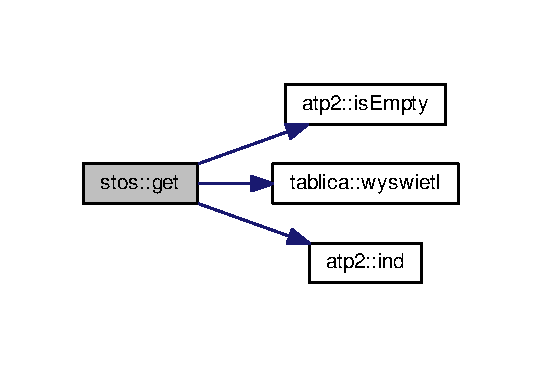
\includegraphics[width=260pt]{classstos_a5d1b9f3ae3c00298385b555113a7467a_cgraph}
\end{center}
\end{figure}


\hypertarget{classstos_a84a6713aeafdd62ef6fe51fa11b7b6fa}{}\index{stos@{stos}!get@{get}}
\index{get@{get}!stos@{stos}}
\subsubsection[{get}]{\setlength{\rightskip}{0pt plus 5cm}int stos\+::get (
\begin{DoxyParamCaption}
{}
\end{DoxyParamCaption}
)}\label{classstos_a84a6713aeafdd62ef6fe51fa11b7b6fa}


metoda get z parametrem int nie powinna byc uzywana, mozliwe jest uzycie jedynie zerowego indeklu, wszystkie inne zwracaja wyjatek,bezpieczniej jest uzywac \hyperlink{classstos_a84a6713aeafdd62ef6fe51fa11b7b6fa}{get()} 



Definicja w linii 27 pliku stos.\+cpp.



Oto graf wywołań dla tej funkcji\+:\nopagebreak
\begin{figure}[H]
\begin{center}
\leavevmode
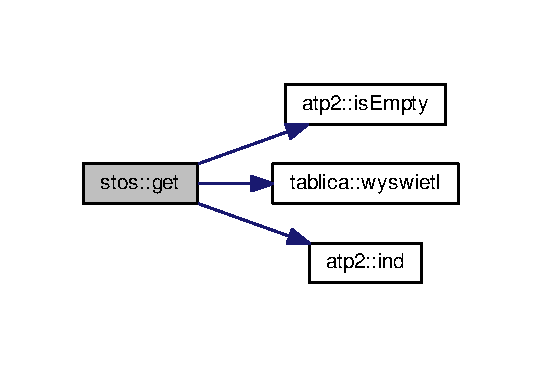
\includegraphics[width=260pt]{classstos_a84a6713aeafdd62ef6fe51fa11b7b6fa_cgraph}
\end{center}
\end{figure}


\hypertarget{classstos_a8af2cbfa1b680a7f045d3390a46a1748}{}\index{stos@{stos}!remove@{remove}}
\index{remove@{remove}!stos@{stos}}
\subsubsection[{remove}]{\setlength{\rightskip}{0pt plus 5cm}void stos\+::remove (
\begin{DoxyParamCaption}
{}
\end{DoxyParamCaption}
)\hspace{0.3cm}{\ttfamily [virtual]}}\label{classstos_a8af2cbfa1b680a7f045d3390a46a1748}


konstruktor bezparametryczny 



Implementuje \hyperlink{classatp_a8294b0364a83890f88ef798b11473f7e}{atp}.



Definicja w linii 9 pliku stos.\+cpp.



Oto graf wywołań dla tej funkcji\+:\nopagebreak
\begin{figure}[H]
\begin{center}
\leavevmode
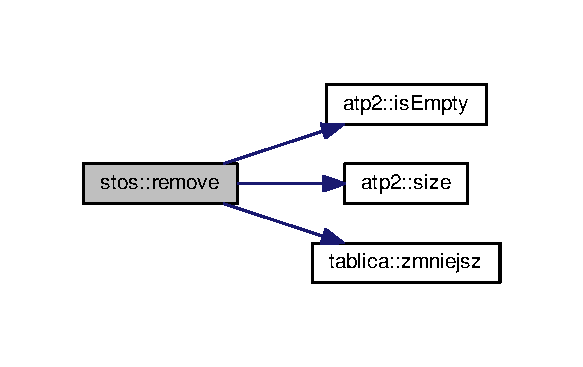
\includegraphics[width=280pt]{classstos_a8af2cbfa1b680a7f045d3390a46a1748_cgraph}
\end{center}
\end{figure}




Dokumentacja dla tej klasy została wygenerowana z plików\+:\begin{DoxyCompactItemize}
\item 
\hyperlink{stos_8hh}{stos.\+hh}\item 
\hyperlink{stos_8cpp}{stos.\+cpp}\end{DoxyCompactItemize}

\hypertarget{classtablica}{}\section{Dokumentacja klasy tablica}
\label{classtablica}\index{tablica@{tablica}}


{\ttfamily \#include $<$tablica.\+hh$>$}



Diagram dziedziczenia dla tablica\nopagebreak
\begin{figure}[H]
\begin{center}
\leavevmode
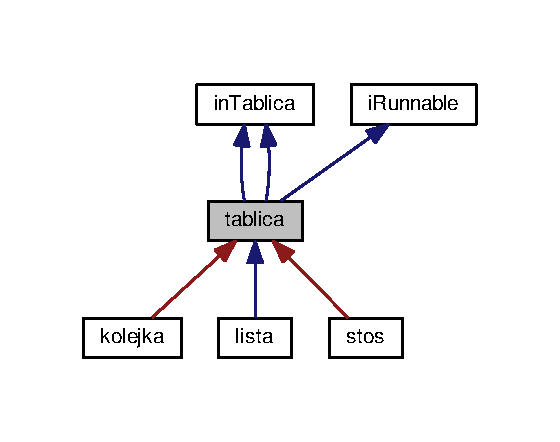
\includegraphics[width=233pt]{classtablica__inherit__graph}
\end{center}
\end{figure}


Diagram współpracy dla tablica\+:\nopagebreak
\begin{figure}[H]
\begin{center}
\leavevmode
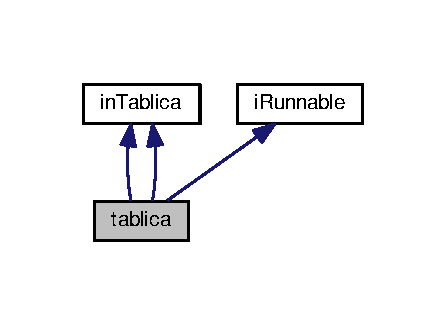
\includegraphics[width=125pt]{classtablica__coll__graph}
\end{center}
\end{figure}
\subsection*{Metody chronione}
\begin{DoxyCompactItemize}
\item 
\hyperlink{classtablica_abc5414ba4d6321ecf744e38a809d9c8f}{tablica} ()
\item 
\hyperlink{classtablica_a5ee1754d39209bec5987d4cbdf19f210}{tablica} (int n)
\item 
int \hyperlink{classtablica_a0c9c746af292f75af844cdd803306fed}{wyswietl} (int n)
\item 
void \hyperlink{classtablica_aa558871f57e678103d92b4038c58623f}{push} (int)
\item 
void \hyperlink{classtablica_af43d08969b1bec83f7abe50f5d76815d}{zwieksz} (int)
\item 
void \hyperlink{classtablica_af615accc61dcccf729ea5f31f03c34e2}{przypisz} (int, int)
\item 
void \hyperlink{classtablica_a5e2094ab2deb4aca91905f96e0f01b08}{zmniejsz} ()
\item 
void \hyperlink{classtablica_aaab8198682dc839a3e99d2fe9a7ae83c}{zdejmij} (int)
\end{DoxyCompactItemize}
\subsection*{Dodatkowe Dziedziczone Składowe}


\subsection{Opis szczegółowy}


Definicja w linii 8 pliku tablica.\+hh.



\subsection{Dokumentacja konstruktora i destruktora}
\hypertarget{classtablica_abc5414ba4d6321ecf744e38a809d9c8f}{}\index{tablica@{tablica}!tablica@{tablica}}
\index{tablica@{tablica}!tablica@{tablica}}
\subsubsection[{tablica}]{\setlength{\rightskip}{0pt plus 5cm}tablica\+::tablica (
\begin{DoxyParamCaption}
{}
\end{DoxyParamCaption}
)\hspace{0.3cm}{\ttfamily [inline]}, {\ttfamily [protected]}}\label{classtablica_abc5414ba4d6321ecf744e38a809d9c8f}


Definicja w linii 16 pliku tablica.\+hh.

\hypertarget{classtablica_a5ee1754d39209bec5987d4cbdf19f210}{}\index{tablica@{tablica}!tablica@{tablica}}
\index{tablica@{tablica}!tablica@{tablica}}
\subsubsection[{tablica}]{\setlength{\rightskip}{0pt plus 5cm}tablica\+::tablica (
\begin{DoxyParamCaption}
\item[{int}]{n}
\end{DoxyParamCaption}
)\hspace{0.3cm}{\ttfamily [inline]}, {\ttfamily [protected]}}\label{classtablica_a5ee1754d39209bec5987d4cbdf19f210}


Definicja w linii 17 pliku tablica.\+hh.



\subsection{Dokumentacja funkcji składowych}
\hypertarget{classtablica_af615accc61dcccf729ea5f31f03c34e2}{}\index{tablica@{tablica}!przypisz@{przypisz}}
\index{przypisz@{przypisz}!tablica@{tablica}}
\subsubsection[{przypisz}]{\setlength{\rightskip}{0pt plus 5cm}void tablica\+::przypisz (
\begin{DoxyParamCaption}
\item[{int}]{dana, }
\item[{int}]{miejsce}
\end{DoxyParamCaption}
)\hspace{0.3cm}{\ttfamily [protected]}}\label{classtablica_af615accc61dcccf729ea5f31f03c34e2}


Definicja w linii 22 pliku tablica.\+cpp.



Oto graf wywoływań tej funkcji\+:\nopagebreak
\begin{figure}[H]
\begin{center}
\leavevmode
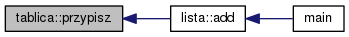
\includegraphics[width=334pt]{classtablica_af615accc61dcccf729ea5f31f03c34e2_icgraph}
\end{center}
\end{figure}


\hypertarget{classtablica_aa558871f57e678103d92b4038c58623f}{}\index{tablica@{tablica}!push@{push}}
\index{push@{push}!tablica@{tablica}}
\subsubsection[{push}]{\setlength{\rightskip}{0pt plus 5cm}void tablica\+::push (
\begin{DoxyParamCaption}
\item[{int}]{dana}
\end{DoxyParamCaption}
)\hspace{0.3cm}{\ttfamily [protected]}}\label{classtablica_aa558871f57e678103d92b4038c58623f}


Definicja w linii 2 pliku tablica.\+cpp.



Oto graf wywołań dla tej funkcji\+:\nopagebreak
\begin{figure}[H]
\begin{center}
\leavevmode
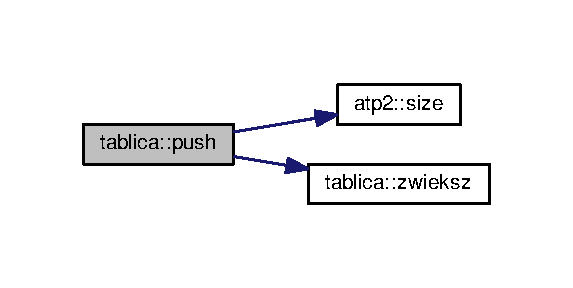
\includegraphics[width=275pt]{classtablica_aa558871f57e678103d92b4038c58623f_cgraph}
\end{center}
\end{figure}




Oto graf wywoływań tej funkcji\+:\nopagebreak
\begin{figure}[H]
\begin{center}
\leavevmode
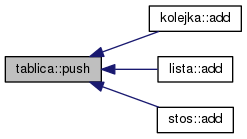
\includegraphics[width=257pt]{classtablica_aa558871f57e678103d92b4038c58623f_icgraph}
\end{center}
\end{figure}


\hypertarget{classtablica_a0c9c746af292f75af844cdd803306fed}{}\index{tablica@{tablica}!wyswietl@{wyswietl}}
\index{wyswietl@{wyswietl}!tablica@{tablica}}
\subsubsection[{wyswietl}]{\setlength{\rightskip}{0pt plus 5cm}int tablica\+::wyswietl (
\begin{DoxyParamCaption}
\item[{int}]{n}
\end{DoxyParamCaption}
)\hspace{0.3cm}{\ttfamily [inline]}, {\ttfamily [protected]}}\label{classtablica_a0c9c746af292f75af844cdd803306fed}


Definicja w linii 19 pliku tablica.\+hh.



Oto graf wywoływań tej funkcji\+:\nopagebreak
\begin{figure}[H]
\begin{center}
\leavevmode
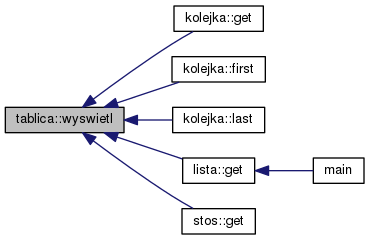
\includegraphics[width=349pt]{classtablica_a0c9c746af292f75af844cdd803306fed_icgraph}
\end{center}
\end{figure}


\hypertarget{classtablica_aaab8198682dc839a3e99d2fe9a7ae83c}{}\index{tablica@{tablica}!zdejmij@{zdejmij}}
\index{zdejmij@{zdejmij}!tablica@{tablica}}
\subsubsection[{zdejmij}]{\setlength{\rightskip}{0pt plus 5cm}void tablica\+::zdejmij (
\begin{DoxyParamCaption}
\item[{int}]{index}
\end{DoxyParamCaption}
)\hspace{0.3cm}{\ttfamily [protected]}}\label{classtablica_aaab8198682dc839a3e99d2fe9a7ae83c}


Definicja w linii 35 pliku tablica.\+cpp.



Oto graf wywołań dla tej funkcji\+:\nopagebreak
\begin{figure}[H]
\begin{center}
\leavevmode
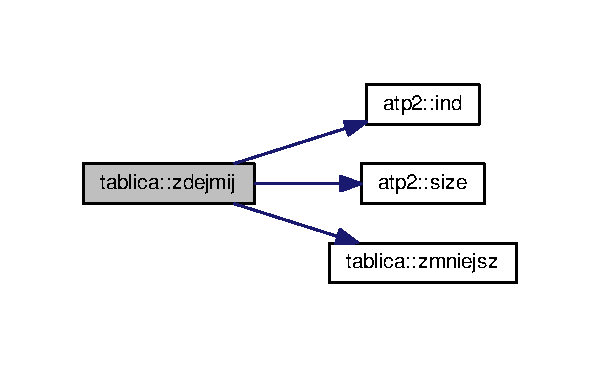
\includegraphics[width=288pt]{classtablica_aaab8198682dc839a3e99d2fe9a7ae83c_cgraph}
\end{center}
\end{figure}




Oto graf wywoływań tej funkcji\+:\nopagebreak
\begin{figure}[H]
\begin{center}
\leavevmode
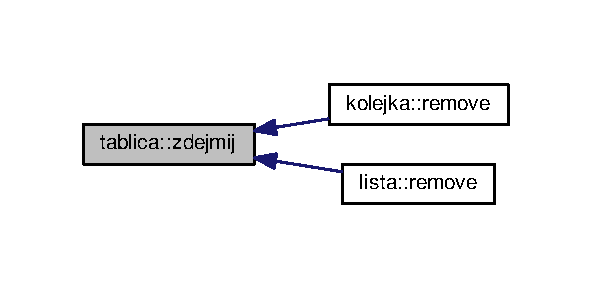
\includegraphics[width=284pt]{classtablica_aaab8198682dc839a3e99d2fe9a7ae83c_icgraph}
\end{center}
\end{figure}


\hypertarget{classtablica_a5e2094ab2deb4aca91905f96e0f01b08}{}\index{tablica@{tablica}!zmniejsz@{zmniejsz}}
\index{zmniejsz@{zmniejsz}!tablica@{tablica}}
\subsubsection[{zmniejsz}]{\setlength{\rightskip}{0pt plus 5cm}void tablica\+::zmniejsz (
\begin{DoxyParamCaption}
{}
\end{DoxyParamCaption}
)\hspace{0.3cm}{\ttfamily [protected]}}\label{classtablica_a5e2094ab2deb4aca91905f96e0f01b08}


Definicja w linii 52 pliku tablica.\+cpp.



Oto graf wywoływań tej funkcji\+:\nopagebreak
\begin{figure}[H]
\begin{center}
\leavevmode
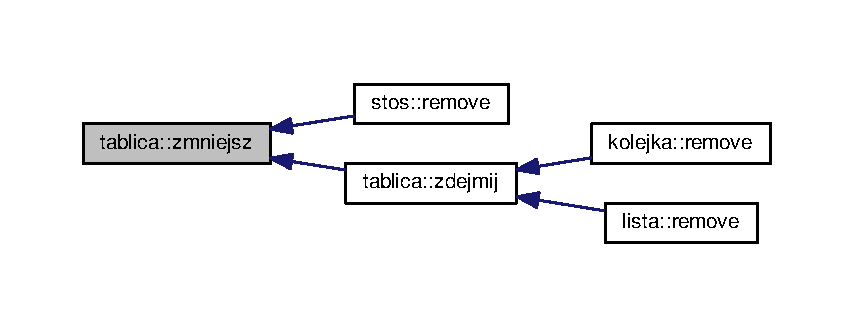
\includegraphics[width=350pt]{classtablica_a5e2094ab2deb4aca91905f96e0f01b08_icgraph}
\end{center}
\end{figure}


\hypertarget{classtablica_af43d08969b1bec83f7abe50f5d76815d}{}\index{tablica@{tablica}!zwieksz@{zwieksz}}
\index{zwieksz@{zwieksz}!tablica@{tablica}}
\subsubsection[{zwieksz}]{\setlength{\rightskip}{0pt plus 5cm}void tablica\+::zwieksz (
\begin{DoxyParamCaption}
\item[{int}]{dana}
\end{DoxyParamCaption}
)\hspace{0.3cm}{\ttfamily [protected]}}\label{classtablica_af43d08969b1bec83f7abe50f5d76815d}


Definicja w linii 10 pliku tablica.\+cpp.



Oto graf wywoływań tej funkcji\+:\nopagebreak
\begin{figure}[H]
\begin{center}
\leavevmode
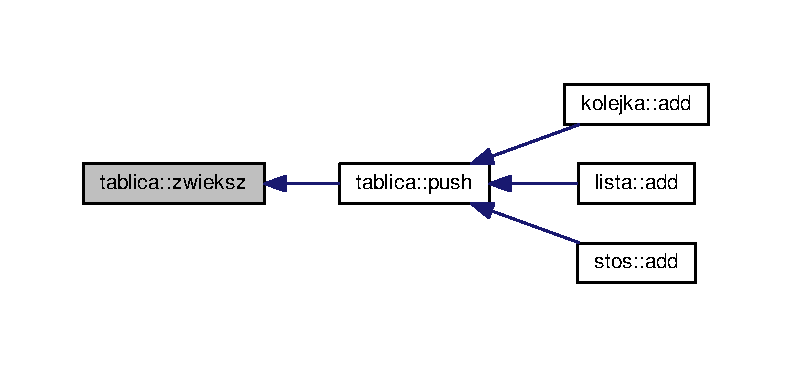
\includegraphics[width=350pt]{classtablica_af43d08969b1bec83f7abe50f5d76815d_icgraph}
\end{center}
\end{figure}




Dokumentacja dla tej klasy została wygenerowana z plików\+:\begin{DoxyCompactItemize}
\item 
\hyperlink{tablica_8hh}{tablica.\+hh}\item 
\hyperlink{tablica_8cpp}{tablica.\+cpp}\end{DoxyCompactItemize}

\chapter{Dokumentacja plików}
\section{Dokumentacja pliku inc/irunnable.hh}
\label{irunnable_8hh}\index{inc/irunnable.\+hh@{inc/irunnable.\+hh}}


zawira interfejs do testowania zaimplementowanych algorytmow  


{\ttfamily \#include \char`\"{}stoper.\+hh\char`\"{}}\\*
{\ttfamily \#include $<$cstdlib$>$}\\*
Wykres zależności załączania dla irunnable.\+hh\+:
\nopagebreak
\begin{figure}[H]
\begin{center}
\leavevmode
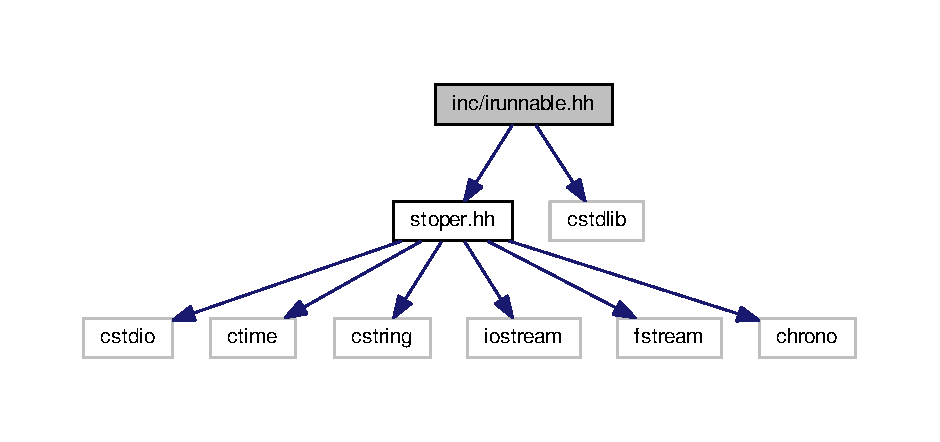
\includegraphics[width=350pt]{irunnable_8hh__incl}
\end{center}
\end{figure}
Ten wykres pokazuje, które pliki bezpośrednio lub pośrednio załączają ten plik\+:
\nopagebreak
\begin{figure}[H]
\begin{center}
\leavevmode
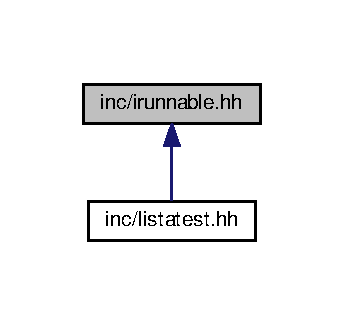
\includegraphics[width=165pt]{irunnable_8hh__dep__incl}
\end{center}
\end{figure}
\subsection*{Komponenty}
\begin{DoxyCompactItemize}
\item 
class {\bf i\+Runnable}
\end{DoxyCompactItemize}


\subsection{Opis szczegółowy}
zawira interfejs do testowania zaimplementowanych algorytmow 


\section{Dokumentacja pliku inc/kolejka.hh}
\label{kolejka_8hh}\index{inc/kolejka.\+hh@{inc/kolejka.\+hh}}


plik zawiera definicje klasy kolejka  


{\ttfamily \#include \char`\"{}tablica.\+hh\char`\"{}}\\*
{\ttfamily \#include \char`\"{}inkolejka.\+hh\char`\"{}}\\*
Wykres zależności załączania dla kolejka.\+hh\+:
\nopagebreak
\begin{figure}[H]
\begin{center}
\leavevmode
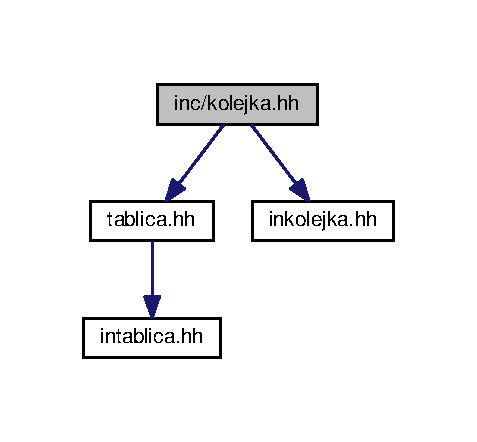
\includegraphics[width=229pt]{kolejka_8hh__incl}
\end{center}
\end{figure}
\subsection*{Komponenty}
\begin{DoxyCompactItemize}
\item 
class {\bf kolejka}
\end{DoxyCompactItemize}


\subsection{Opis szczegółowy}
plik zawiera definicje klasy kolejka 


\hypertarget{lista_8hh}{}\section{Dokumentacja pliku lista.\+hh}
\label{lista_8hh}\index{lista.\+hh@{lista.\+hh}}


plik zawiera klase lista  


{\ttfamily \#include \char`\"{}tablica.\+hh\char`\"{}}\\*
Wykres zależności załączania dla lista.\+hh\+:\nopagebreak
\begin{figure}[H]
\begin{center}
\leavevmode
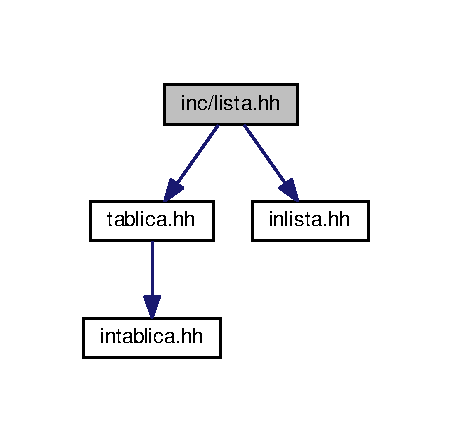
\includegraphics[width=139pt]{lista_8hh__incl}
\end{center}
\end{figure}
\subsection*{Komponenty}
\begin{DoxyCompactItemize}
\item 
class \hyperlink{classlista}{lista}
\end{DoxyCompactItemize}


\subsection{Opis szczegółowy}
plik zawiera klase lista 


\section{Dokumentacja pliku inc/listatest.hh}
\label{listatest_8hh}\index{inc/listatest.\+hh@{inc/listatest.\+hh}}


plik zawiera klase listatest  


{\ttfamily \#include \char`\"{}tablicatest.\+hh\char`\"{}}\\*
{\ttfamily \#include \char`\"{}inlista.\+hh\char`\"{}}\\*
{\ttfamily \#include \char`\"{}irunnable.\+hh\char`\"{}}\\*
Wykres zależności załączania dla listatest.\+hh\+:
\nopagebreak
\begin{figure}[H]
\begin{center}
\leavevmode
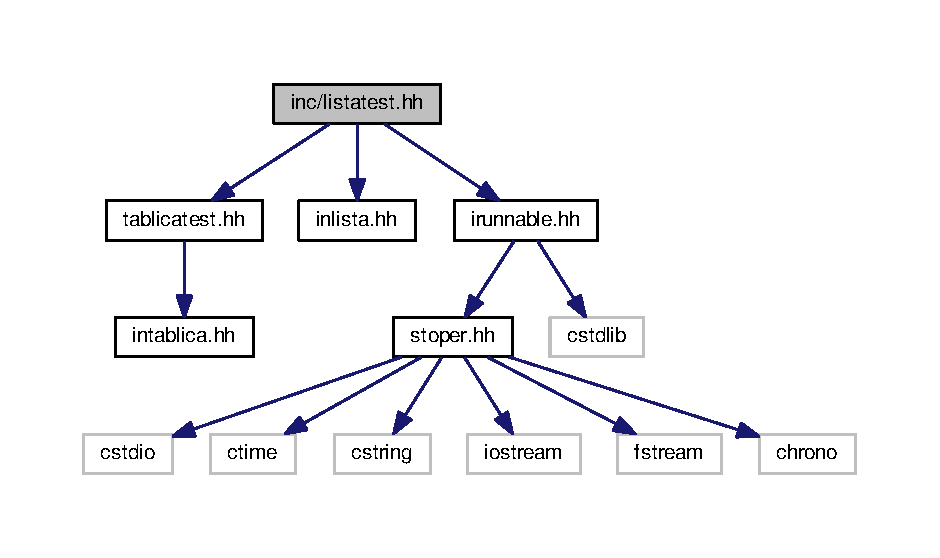
\includegraphics[width=350pt]{listatest_8hh__incl}
\end{center}
\end{figure}
\subsection*{Komponenty}
\begin{DoxyCompactItemize}
\item 
class {\bf listatest}
\end{DoxyCompactItemize}


\subsection{Opis szczegółowy}
plik zawiera klase listatest 


\section{Dokumentacja pliku inc/sort.hh}
\label{sort_8hh}\index{inc/sort.\+hh@{inc/sort.\+hh}}


plik zawiera funkcje z metodami sortowania  


\subsection*{Funkcje}
\begin{DoxyCompactItemize}
\item 
void {\bfseries bubblesort} (int tab[$\,$], int size)\label{sort_8hh_ad362c6069fd79ce1dd0ce9c3db15fdd7}

\end{DoxyCompactItemize}


\subsection{Opis szczegółowy}
plik zawiera funkcje z metodami sortowania 


\section{Dokumentacja pliku inc/stos.hh}
\label{stos_8hh}\index{inc/stos.\+hh@{inc/stos.\+hh}}


plik zawiera definicje klasy stos  


{\ttfamily \#include \char`\"{}tablica.\+hh\char`\"{}}\\*
{\ttfamily \#include \char`\"{}instos.\+hh\char`\"{}}\\*
Wykres zależności załączania dla stos.\+hh\+:
\nopagebreak
\begin{figure}[H]
\begin{center}
\leavevmode
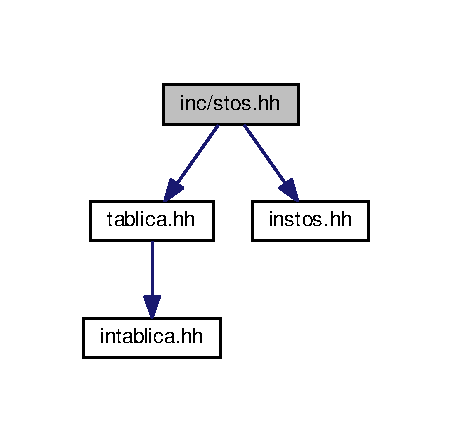
\includegraphics[width=217pt]{stos_8hh__incl}
\end{center}
\end{figure}
\subsection*{Komponenty}
\begin{DoxyCompactItemize}
\item 
class {\bf stos}
\end{DoxyCompactItemize}


\subsection{Opis szczegółowy}
plik zawiera definicje klasy stos 


\hypertarget{tablica_8hh}{}\section{Dokumentacja pliku tablica.\+hh}
\label{tablica_8hh}\index{tablica.\+hh@{tablica.\+hh}}


plik zawiera klase tablica  


{\ttfamily \#include \char`\"{}atp2.\+hh\char`\"{}}\\*
Wykres zależności załączania dla tablica.\+hh\+:\nopagebreak
\begin{figure}[H]
\begin{center}
\leavevmode
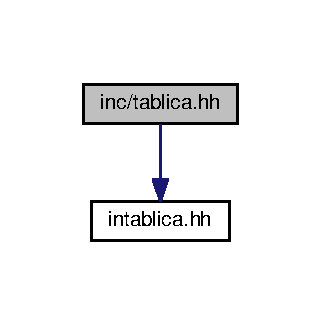
\includegraphics[width=139pt]{tablica_8hh__incl}
\end{center}
\end{figure}
Ten wykres pokazuje, które pliki bezpośrednio lub pośrednio załączają ten plik\+:
\nopagebreak
\begin{figure}[H]
\begin{center}
\leavevmode
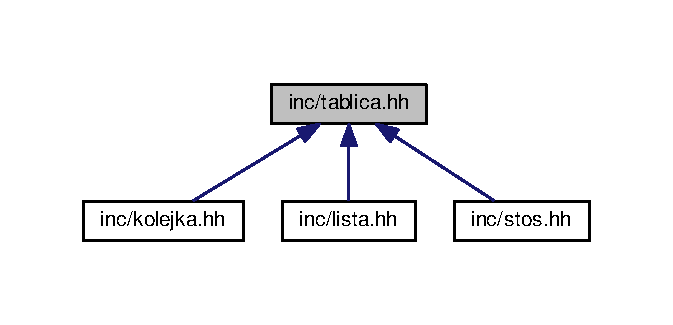
\includegraphics[width=275pt]{tablica_8hh__dep__incl}
\end{center}
\end{figure}
\subsection*{Komponenty}
\begin{DoxyCompactItemize}
\item 
class \hyperlink{classtablica}{tablica}
\end{DoxyCompactItemize}


\subsection{Opis szczegółowy}
plik zawiera klase tablica 


\section{Dokumentacja pliku inc/tablicatest.hh}
\label{tablicatest_8hh}\index{inc/tablicatest.\+hh@{inc/tablicatest.\+hh}}


plik zawiera klase tablicatest  


{\ttfamily \#include \char`\"{}intablica.\+hh\char`\"{}}\\*
Wykres zależności załączania dla tablicatest.\+hh\+:
\nopagebreak
\begin{figure}[H]
\begin{center}
\leavevmode
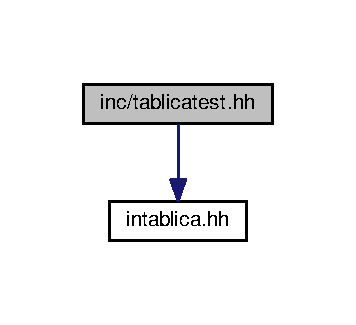
\includegraphics[width=171pt]{tablicatest_8hh__incl}
\end{center}
\end{figure}
Ten wykres pokazuje, które pliki bezpośrednio lub pośrednio załączają ten plik\+:
\nopagebreak
\begin{figure}[H]
\begin{center}
\leavevmode
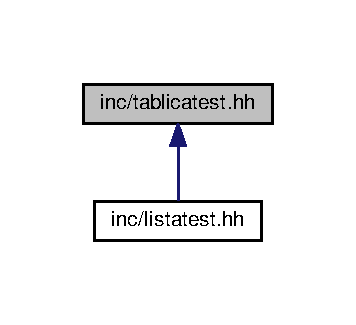
\includegraphics[width=171pt]{tablicatest_8hh__dep__incl}
\end{center}
\end{figure}
\subsection*{Komponenty}
\begin{DoxyCompactItemize}
\item 
class {\bf tablica}
\item 
class {\bf tablica\+::empty}
\begin{DoxyCompactList}\small\item\em metoda sprawdza czy kontener jest pusty \end{DoxyCompactList}\item 
class {\bf tablica\+::bad\+\_\+index}
\begin{DoxyCompactList}\small\item\em obiekt zwracany podczas wystapienia wyjatku wystepujacego gdy nastapi proba odzialywania na dane ktorych kontener nie posiada \end{DoxyCompactList}\end{DoxyCompactItemize}


\subsection{Opis szczegółowy}
plik zawiera klase tablicatest 


%--- End generated contents ---

% Index
\backmatter
\newpage
\phantomsection
\clearemptydoublepage
\addcontentsline{toc}{chapter}{Indeks}
\printindex

\end{document}
